\documentclass[11pt,a4paper]{report}
\usepackage[utf8]{inputenc}
\usepackage{geometry}
\geometry{margin=1in}
\usepackage{graphicx}
\usepackage{setspace}
\usepackage{titlesec}
\usepackage{longtable}
\usepackage{booktabs}
\usepackage{amsmath}
\usepackage{tikz}
\usetikzlibrary{arrows.meta,positioning}
\usepackage[hidelinks]{hyperref}

\setcounter{secnumdepth}{3}
\renewcommand{\thesection}{\arabic{section}}

\begin{document}

% ------------------ Title Page (template structure retained) ------------------
\begin{titlepage}
    \centering
    
\includegraphics[width=3.4cm,height=2.6cm]{college_logo.jpg}\\[0.5cm]
    \vspace{1cm}
    \textbf{\large A Course End Project Report on} \\[0.5cm]
    {\LARGE \textbf{Bank Account Management System}}\\[1.5cm]
    \textbf{Submitted by}\\[0.25cm]
    Batch No. 7
    \begin{center}
        \setstretch{1}
        \begin{tabular}{l l}
            {D Taraka Ramarao} & {25881A05EH} \\ [2mm]
        \end{tabular}
    \end{center}
    \textbf{Course Facilitator}\\[0.075in]
    {Mr. D Ganesh Deshmukh}\\[3cm]
    {\large\textbf{Department of Computer Science and Engineering (CSE)}}\\[0.5cm]
    {\large\textbf{Vardhaman College of Engineering, Hyderabad}}\\[0.5cm]
    {\large \textbf{October 2025}}
\end{titlepage}

\tableofcontents
\newpage

\section*{Abstract}
\noindent Manual, paper-based handling of bank accounts is slow, error-prone, and makes it hard to keep a reliable history of deposits, withdrawals, and transfers. This project implements a Bank Account Management System as a Java desktop application with a Swing graphical interface. A user can create savings and current accounts, deposit and withdraw money, transfer funds between accounts, apply interest to savings accounts, search accounts by holder name, view a transaction history, and close a zero-balance account. All data is stored in plain CSV files, so the system runs with only a Java Development Kit (JDK) and no database server or external library.

The implementation separates concerns into model, service, persistence, and user-interface layers. Money is represented with \texttt{BigDecimal} rather than floating-point types, business rules are enforced in a single service class, and every successful movement is recorded as a transaction before the data is saved. A dependency-free automated test suite covering creation, deposits, withdrawals, transfers, interest, closure, search, and persistence reload was run against the final code: 24 checks passed and 0 failed. The compiled report, source code, tests, screenshot, and build scripts in this submission all describe the same, actually built system.

\textbf{Keywords}: bank account management, Java, Swing, BigDecimal, CSV persistence, software testing.

\section{Introduction}
A bank account is, at its core, a small set of operations that must never go wrong: money in, money out, money moved between accounts, and an accurate record of each step. Real banking systems add authentication, networking, and regulation on top of this core, but the core itself must already guarantee that a balance cannot go negative, that a failed operation leaves balances unchanged, and that history is not lost when the program closes.

\subsection{Problem Statement}
Small-scale account handling is often taught or prototyped with spreadsheets or ad-hoc console programs. Those approaches have three recurring weaknesses. First, validation is scattered or missing, so a negative deposit or an overdrawn withdrawal can corrupt a balance. Second, money is frequently stored as a floating-point number, which cannot represent decimal currency exactly. Third, transaction history is either absent or kept only in memory, so it disappears when the program exits. This project addresses those three weaknesses directly, in a system small enough to be understood, tested, and extended.

\subsection{Scope}
The system is a single-user desktop application. It covers account creation, deposit, withdrawal, transfer, savings interest, search, transaction history, account closure, and file persistence. It does not cover user login, networked or multi-user access, online payments, or connection to a real bank; those are listed as future work in Section~\ref{sec:limitations} rather than claimed as implemented features.

\section{Existing Approach and Proposed Solution}
Existing teaching examples of bank systems commonly use a console menu, store balances in memory, and use \texttt{double} for money. That is adequate for a first exercise, but it leaves the three weaknesses above unresolved and gives the user no persistent record.

The proposed solution keeps the same familiar operations and improves the engineering underneath them:
\begin{itemize}
    \item A Swing window replaces the console menu, showing all accounts in a table and the selected account's history below it.
    \item \texttt{BigDecimal} with scale 2 represents every amount, so 0.10 is stored exactly.
    \item One service class owns every rule, so the interface cannot bypass validation.
    \item Two CSV files (\texttt{accounts.csv} and \texttt{transactions.csv}) persist accounts and history across runs, with quoted fields for names containing commas.
    \item A test suite exercises the service directly, without a display, so the rules are verified independently of the interface.
\end{itemize}

\section{Objectives}
\begin{itemize}
    \item To build a working desktop system for creating and managing bank accounts.
    \item To implement deposit, withdrawal, transfer, interest, search, history, and closure correctly.
    \item To prevent invalid operations: non-positive amounts, overdrafts, transfers to the same account, operations on closed accounts, and closure of a non-empty account.
    \item To persist accounts and transaction history in files that survive a restart.
    \item To verify the system with automated tests and a genuine screenshot of the running application.
    \item To document the system accurately, without claiming features that were not built.
\end{itemize}

\section{Requirements and Technology Stack}
\subsection{Functional Requirements}
\begin{enumerate}
    \item Create a savings or current account with a holder name and an optional opening deposit.
    \item Deposit to, and withdraw from, an account by account number.
    \item Transfer an amount between two different, active accounts.
    \item Apply simple interest to a savings account at a stated annual percentage rate.
    \item List all accounts, search by holder name (case-insensitive), and view an account's transactions.
    \item Close an account only when its balance is zero; closed accounts accept no further operations.
    \item Save every change to disk and reload the same state on the next run.
\end{enumerate}

\subsection{Non-Functional Requirements}
The system must start with only a JDK, must not require a database server, must reject invalid input with a readable error message rather than crashing, and must keep balances exact to two decimal places. The interface must remain usable without training beyond the labelled buttons.

\subsection{Technology Stack}
\begin{table}[h]
    \centering
    \caption{Technology stack, as actually used}
    \begin{tabular}{p{4cm}p{10cm}}
        \toprule
        \textbf{Item} & \textbf{Choice and reason} \\
        \midrule
        Language & Java, compiled with \texttt{--release 17} (runs on JDK 17 or later; developed and tested here on JDK 21). \\
        Interface & Java Swing (standard library, no extra GUI framework). \\
        Money & \texttt{java.math.BigDecimal}, scale 2, rounding \texttt{HALF\_UP}. \\
        Persistence & Plain CSV files read and written with the standard library; no database, no external dependency. \\
        Build & \texttt{javac} directly, driven by \texttt{compile.sh}, \texttt{run.sh}, and \texttt{test.sh}. No Maven or Gradle is required. \\
        Tests & A dependency-free Java test runner (see Section~\ref{sec:testing}). \\
        Report & \LaTeX\ (pdf\LaTeX, TeX Live), based on the supplied course-end template. \\
        \bottomrule
    \end{tabular}
\end{table}

\section{System Architecture and Module Description}
The design follows a simple layered structure. The interface never touches files or balances directly; it calls the service, the service enforces the rules and records transactions, and the store only reads and writes CSV text. This separation is what allows the tests to verify the rules without launching a window.

\begin{figure}[h]
    \centering
    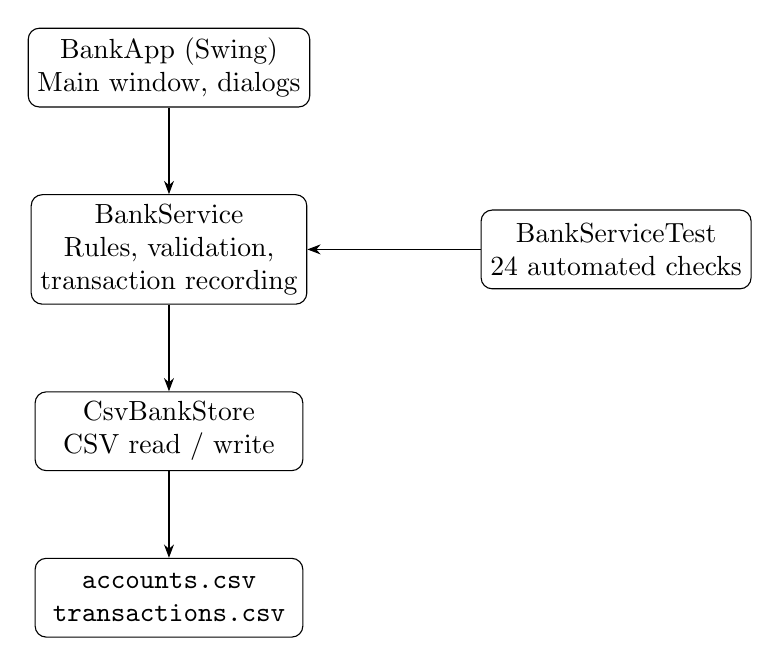
\begin{tikzpicture}[node distance=1.1cm, box/.style={draw, rounded corners, align=center, minimum width=3.4cm, minimum height=1.0cm}, arrow/.style={-{Stealth}}]
        \node[box] (ui) {BankApp (Swing)\\Main window, dialogs};
        \node[box, below=of ui] (svc) {BankService\\Rules, validation,\\transaction recording};
        \node[box, below=of svc] (store) {CsvBankStore\\CSV read / write};
        \node[box, below=of store] (files) {\texttt{accounts.csv}\\\texttt{transactions.csv}};
        \node[box, right=2.2cm of svc] (tests) {BankServiceTest\\24 automated checks};
        \draw[arrow] (ui) -- (svc);
        \draw[arrow] (svc) -- (store);
        \draw[arrow] (store) -- (files);
        \draw[arrow] (tests) -- (svc);
    \end{tikzpicture}
    \caption{Layered architecture. Arrows show which layer calls which; tests exercise the service directly.}
    \label{fig:architecture}
\end{figure}

\begin{table}[h]
    \centering
    \caption{Modules and their responsibilities}
    \begin{tabular}{p{4.5cm}p{9.5cm}}
        \toprule
        \textbf{Module (package)} & \textbf{Responsibility} \\
        \midrule
        \texttt{model} & \texttt{Account}, \texttt{Transaction}, \texttt{AccountType}, \texttt{TransactionType}: state only, no business rules. \\
        \texttt{service.BankService} & All rules in Section~\ref{sec:design}: validation, transfers, interest, closure, search, and saving after each change. \\
        \texttt{CsvBankStore} (persistence) & Loads and saves the two CSV files, including quoting for commas and quotes in names and notes. \\
        \texttt{ui.BankApp} & Swing window, account table, history pane, input dialogs, and error messages. \\
        \texttt{Main} & Entry point, delegates to \texttt{BankApp}. \\
        \texttt{tests} & \texttt{BankServiceTest}: the automated suite, run by \texttt{test.sh}. \\
        \bottomrule
    \end{tabular}
\end{table}

\section{Design, Algorithms, and Workflows}
\label{sec:design}
\subsection{Data Structures}
Accounts are kept in a \texttt{LinkedHashMap} keyed by account number, which gives constant-time lookup by number while preserving creation order for listing. Transactions are kept in an \texttt{ArrayList} in creation order; history for one account is obtained by filtering that list. Account numbers are sequential, starting at 1001, and the next number is recomputed from the largest stored number on load, so numbers are never reused after a restart. Transaction identifiers are sequential in the same way.

\subsection{Key Workflows}
\textbf{Deposit / withdrawal.} Validate that the account exists and is active, validate that the amount is positive, and for a withdrawal check that the balance covers it. Only then change the balance, append a transaction recording the balance after the movement, and save both files. A rejected operation changes nothing.

\textbf{Transfer.} This is the operation most vulnerable to partial failure, so all checks come first: the two accounts must differ, both must exist and be active, the amount must be positive, and the source balance must cover it. Only after every check passes are both balances changed, with a \texttt{TRANSFER\_OUT} entry for the source and a \texttt{TRANSFER\_IN} entry for the destination, followed by a save. A failed transfer therefore leaves both accounts untouched, which the tests verify.

\textbf{Interest.} Interest applies only to savings accounts. It is simple interest on the current balance: $\text{interest} = \text{balance} \times \text{rate} / 100$, rounded to two decimal places. A current account requesting interest is rejected, and a zero interest amount records nothing.

\textbf{Closure and search.} Closure requires an active account with an exactly zero balance; otherwise the user is told to withdraw the balance first. Search matches holder names case-insensitively by substring and returns an empty list, not an error, when nothing matches.

\subsection{Validation Example}
The withdrawal rule, in simplified form, is: reject a non-positive amount, reject an unknown or closed account, reject an amount above the balance, and only then subtract and record. The same ordering (validate everything, then mutate, then record, then save) is used for every movement in the system.

\section{Implementation Details}
The project contains no external dependencies, so there is nothing to download before building. Compilation is a single \texttt{javac} invocation over the files under \texttt{src/}. The data directory defaults to \texttt{data/} in the working directory and can be overridden with the system property \texttt{bank.data.dir}, which is how the screenshot data was kept separate from a user's real data.

File format is deliberately readable: one account per line in \texttt{accounts.csv} (number, holder, type, balance, active, created timestamp) and one transaction per line in \texttt{transactions.csv} (identifier, account number, type, amount, balance after, timestamp, note). A user can inspect these files in any text editor, and the store's CSV quoting handles holder names that contain commas.

Two defects were found and fixed during development, and are recorded here because they affected the delivered code. First, the account setters were package-private while the service lives in a different package, which failed compilation; the setters were made public with the service as their only caller. Second, a Swing field-initialisation ordering error (a button action referring to the search field before it was created) failed compilation; the field is now created before the button panel. Both fixes were verified by a clean recompilation and a full test run.

\section{User Interface and Screenshot}
The main window (Figure~\ref{fig:ui}) shows the account table at the top, with Create Account, Deposit, Withdraw, Transfer, Apply Interest, Close Account, Refresh, and search controls, and the selected account's transaction history below. Invalid operations show the service's error message in a dialog instead of crashing the window.

\begin{figure}[htbp]
    \centering
    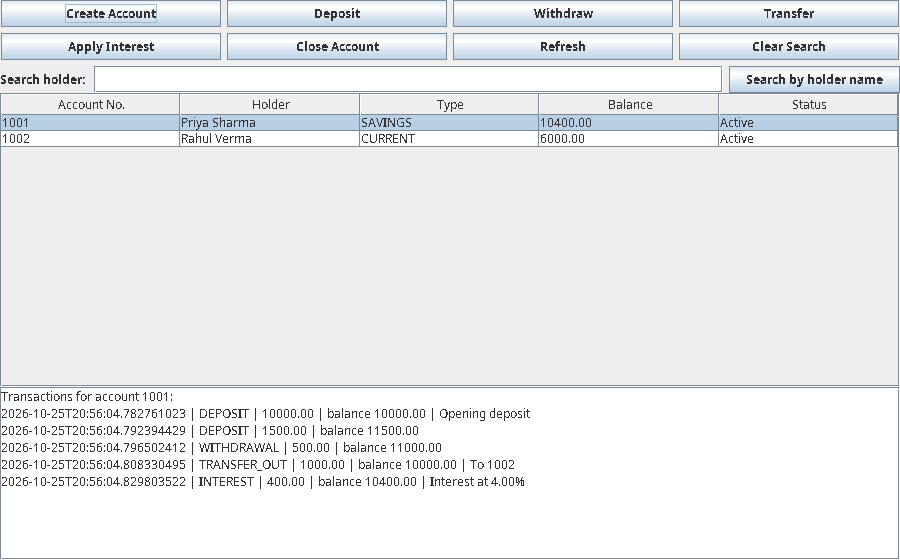
\includegraphics[width=\linewidth]{main_window.png}
    \caption{Genuine screenshot of the running application under Xvfb, captured with \texttt{java.awt.Robot}. The demo data (sample holders Priya Sharma and Rahul Verma) was created through the real \texttt{BankService}: account 1001, a savings account, shows an opening deposit of 10000.00, a deposit of 1500.00, a withdrawal of 500.00, a transfer out of 1000.00, and 4\% interest of 400.00, ending at 10400.00; account 1002 ends at 6000.00 after receiving the transfer. These are sample names for demonstration, not real customers.}
    \label{fig:ui}
\end{figure}

\section{Testing Methodology and Results}
\label{sec:testing}
\subsection{Methodology}
Testing is done at the service layer, where the rules live, so a test failure points at a rule rather than at the interface. The suite in \texttt{tests/com/bank/BankServiceTest.java} uses no external library: each check prints PASS or FAIL, and the process exits non-zero if any check fails. Tests run against a temporary directory, so they never touch a user's real \texttt{data/} folder. In addition to the suite, the full application was launched under Xvfb and its window captured (Figure~\ref{fig:ui}), and the demo data was reloaded to confirm persistence.

\subsection{Test Cases and Actual Results}
\begin{table}[h]
    \centering
    \caption{Automated test results for the final code (run with \texttt{./test.sh}, JDK 21)}
    \begin{tabular}{p{8.5cm}c}
        \toprule
        \textbf{Check} & \textbf{Result} \\
        \midrule
        Account creation, first number 1001, opening balance & Pass \\
        Deposit and withdrawal change the balance correctly & Pass \\
        Withdrawal above balance rejected; balance unchanged & Pass \\
        Negative deposit, zero withdrawal, unknown account rejected & Pass \\
        Second account numbered sequentially (1002) & Pass \\
        Transfer debits source and credits destination & Pass \\
        Transfer to same account, and transfer above balance, rejected & Pass \\
        4\% interest on 1000.00 gives 1040.00; interest on current account rejected & Pass \\
        Non-zero account cannot close; zero-balance account closes; closed account rejects deposits & Pass \\
        Case-insensitive name search; empty result for no match & Pass \\
        Reload from CSV preserves balances, closed status, and history & Pass \\
        \bottomrule
    \end{tabular}
\end{table}

\noindent The suite reported \textbf{24 passed, 0 failed}. The compilation command (\texttt{./compile.sh}, \texttt{javac --release 17}) also succeeded, and the GUI launch under Xvfb produced the screenshot in Figure~\ref{fig:ui} without an error. No test, metric, or screenshot in this report was fabricated: the numbers above are the output of the runs just described.

\section{Limitations and Future Improvements}
\label{sec:limitations}
\begin{itemize}
    \item \textbf{Single user, no authentication.} Anyone who can run the program can operate any account. A login and per-user ownership check would be required before any real use.
    \item \textbf{No database or concurrency control.} CSV files suit a single user, but concurrent writers could overwrite each other. A database with transactions would be the next step.
    \item \textbf{No network access.} Accounts exist only on one machine; there is no client--server or online-banking layer.
    \item \textbf{Simple interest only, on demand.} Interest is applied when the user asks, not automatically on a schedule, and no fees, overdraft facility, or statement export are implemented.
    \item \textbf{Basic interface.} The Swing interface is functional but plain; input dialogs could be replaced with a dedicated form, and amounts are entered as text.
\end{itemize}
Future work, in priority order, would be authentication, a database-backed store with proper transactions, scheduled interest, statement export (PDF/CSV), and a more polished account form. None of these is claimed as present in this version.

\section{Conclusion}
This project delivers a complete, working Bank Account Management System: a Swing desktop application backed by a small, well-tested service layer and plain CSV persistence. It implements the operations a bank account actually needs, enforces the rules that keep balances consistent (positive amounts, no overdrafts, atomic transfers, savings-only interest, zero-balance closure), records every movement, and survives restarts. The claim is supported by evidence rather than assertion: the code compiles with \texttt{javac}, 24 automated checks pass, and a genuine screenshot shows the running system with a consistent transaction history. The system is intentionally small and dependency-free, which makes it a sound base for the database, authentication, and reporting improvements listed above.

\section{Mapping POs and SDGs}
\subsection{Program Outcomes (POs) Mapping}
\begin{table}[h]
    \centering
    \caption{Mapping of Program Outcomes (POs) to project relevance}
    \begin{tabular}{|c|p{6cm}|p{6cm}|}
        \hline
        \textbf{PO No.} & \textbf{Program Outcome} & \textbf{Relevance} \\
        \hline
        PO1 & Engineering Knowledge & Applied Java, data structures, and decimal arithmetic. \\
        \hline
        PO2 & Problem Analysis & Identified validation, precision, and persistence failures in naive designs. \\
        \hline
        PO3 & Design/Development of Solutions & Designed a layered, tested, working system. \\
        \hline
        PO5 & Modern Tool Usage & Used the JDK, Swing, \LaTeX, and automated testing. \\
        \hline
        PO6 & Engineer and Society & Provides a correct, auditable record of people's money movements. \\
        \hline
    \end{tabular}
\end{table}

\subsection{Sustainable Development Goals (SDGs) Mapping}
\begin{table}[h]
    \centering
    \caption{Mapping of Sustainable Development Goals (SDGs) to project relevance}
    \begin{tabular}{|c|p{6cm}|p{6cm}|}
        \hline
        \textbf{SDG No.} & \textbf{Goal} & \textbf{Relevance} \\
        \hline
        SDG 8 & Decent Work and Economic Growth & Reliable account records support financial participation. \\
        \hline
        SDG 9 & Industry, Innovation, and Infrastructure & A maintainable software system built on standard tools. \\
        \hline
    \end{tabular}
\end{table}

\begin{thebibliography}{99}
\addcontentsline{toc}{section}{Bibliography}
\bibitem{oracle-java}
Oracle, ``Java Platform, Standard Edition Documentation,'' \url{https://docs.oracle.com/en/java/}.
\bibitem{bloch2018}
J. Bloch, \textit{Effective Java}, 3rd ed. Addison-Wesley, 2018.
\bibitem{gamma1994}
E. Gamma, R. Helm, R. Johnson, and J. Vlissides, \textit{Design Patterns: Elements of Reusable Object-Oriented Software}. Addison-Wesley, 1994.
\bibitem{horstmann2019}
C. S. Horstmann, \textit{Core Java, Volume I: Fundamentals}, 11th ed. Pearson, 2019.
\bibitem{lamport1994}
L. Lamport, \textit{\LaTeX: A Document Preparation System}, 2nd ed. Addison-Wesley, 1994.
\end{thebibliography}

\end{document}
